\documentclass{article}
\PassOptionsToPackage{numbers,sort&compress}{natbib}
\usepackage{neurips_2026}
\usepackage[utf8]{inputenc}
\usepackage[T1]{fontenc}
\usepackage{courier} % vector Type-1 monospace; no bitmap EC fonts
\usepackage{amsmath,amsfonts,amssymb,booktabs,graphicx,microtype,url,xcolor}
\usepackage{hyperref}
\hypersetup{colorlinks=true,linkcolor=blue,citecolor=blue,urlcolor=blue}
\expandafter\def\csname resultarenamargin\endcsname{0.004}
\expandafter\def\csname resultarenase\endcsname{0.055}
\expandafter\def\csname resultarenacilow\endcsname{-0.103}
\expandafter\def\csname resultarenacihigh\endcsname{0.106}
\expandafter\def\csname resultarenabootstrapwinnerretention\endcsname{0.520}
\expandafter\def\csname resultarenamarginse\endcsname{0.076}
\expandafter\def\csname resultmthumanmargin\endcsname{0.378}
\expandafter\def\csname resultmthumanse\endcsname{0.136}
\expandafter\def\csname resultmthumancilow\endcsname{0.108}
\expandafter\def\csname resultmthumancihigh\endcsname{0.661}
\expandafter\def\csname resultmthumanbootstrapwinnerretention\endcsname{1.000}
\expandafter\def\csname resultmthumanmarginse\endcsname{2.782}
\expandafter\def\csname resultmtgpt4margin\endcsname{0.820}
\expandafter\def\csname resultmtgpt4se\endcsname{0.153}
\expandafter\def\csname resultmtgpt4cilow\endcsname{0.544}
\expandafter\def\csname resultmtgpt4cihigh\endcsname{1.129}
\expandafter\def\csname resultmtgpt4bootstrapwinnerretention\endcsname{1.000}
\expandafter\def\csname resultmtgpt4marginse\endcsname{5.355}
\expandafter\def\csname resultmthumanmatchedmargin\endcsname{0.293}
\expandafter\def\csname resultmthumanmatchedse\endcsname{0.119}
\expandafter\def\csname resultmthumanmatchedcilow\endcsname{0.084}
\expandafter\def\csname resultmthumanmatchedcihigh\endcsname{0.540}
\expandafter\def\csname resultmthumanmatchedbootstrapwinnerretention\endcsname{0.993}
\expandafter\def\csname resultmthumanmatchedmarginse\endcsname{2.467}
\expandafter\def\csname resultmtgpt4matchedmargin\endcsname{0.772}
\expandafter\def\csname resultmtgpt4matchedse\endcsname{0.168}
\expandafter\def\csname resultmtgpt4matchedcilow\endcsname{0.488}
\expandafter\def\csname resultmtgpt4matchedcihigh\endcsname{1.099}
\expandafter\def\csname resultmtgpt4matchedbootstrapwinnerretention\endcsname{1.000}
\expandafter\def\csname resultmtgpt4matchedmarginse\endcsname{4.604}
\expandafter\def\csname resultnba2013margin\endcsname{0.228}
\expandafter\def\csname resultnba2013se\endcsname{0.324}
\expandafter\def\csname resultnba2013cilow\endcsname{-0.409}
\expandafter\def\csname resultnba2013cihigh\endcsname{0.845}
\expandafter\def\csname resultnba2013bootstrapwinnerretention\endcsname{0.647}
\expandafter\def\csname resultnba2013marginse\endcsname{0.704}
\expandafter\def\csname resultnba2014margin\endcsname{0.295}
\expandafter\def\csname resultnba2014se\endcsname{0.318}
\expandafter\def\csname resultnba2014cilow\endcsname{-0.340}
\expandafter\def\csname resultnba2014cihigh\endcsname{0.930}
\expandafter\def\csname resultnba2014bootstrapwinnerretention\endcsname{0.783}
\expandafter\def\csname resultnba2014marginse\endcsname{0.927}
\expandafter\def\csname resultnba2015margin\endcsname{0.744}
\expandafter\def\csname resultnba2015se\endcsname{0.314}
\expandafter\def\csname resultnba2015cilow\endcsname{0.159}
\expandafter\def\csname resultnba2015cihigh\endcsname{1.386}
\expandafter\def\csname resultnba2015bootstrapwinnerretention\endcsname{0.967}
\expandafter\def\csname resultnba2015marginse\endcsname{2.370}
\expandafter\def\csname resultarenainfluenceedits\endcsname{574}
\expandafter\def\csname resultarenainfluencemaxincidentfraction\endcsname{17.41}
\expandafter\def\csname resultarenainfluencemargin\endcsname{-1.244}
\expandafter\def\csname resultarenainfluencestandardizedreduction\endcsname{22.494}
\expandafter\def\csname resultarenainfluencemarginreduction\endcsname{1.248}
\expandafter\def\csname resultarenaexposurecapedits\endcsname{555}
\expandafter\def\csname resultarenaexposurecapmaxincidentfraction\endcsname{1.00}
\expandafter\def\csname resultarenaexposurecapmargin\endcsname{-0.100}
\expandafter\def\csname resultarenaexposurecapstandardizedreduction\endcsname{1.881}
\expandafter\def\csname resultarenaexposurecapmarginreduction\endcsname{0.104}
\expandafter\def\csname resultarenaamipdeleteedits\endcsname{574}
\expandafter\def\csname resultarenaamipdeletemaxincidentfraction\endcsname{42.84}
\expandafter\def\csname resultarenaamipdeletemargin\endcsname{-2.277}
\expandafter\def\csname resultarenaamipdeletestandardizedreduction\endcsname{41.124}
\expandafter\def\csname resultarenaamipdeletemarginreduction\endcsname{2.281}
\expandafter\def\csname resultmthumaninfluenceedits\endcsname{33}
\expandafter\def\csname resultmthumaninfluencemaxincidentfraction\endcsname{3.31}
\expandafter\def\csname resultmthumaninfluencemargin\endcsname{0.101}
\expandafter\def\csname resultmthumaninfluencestandardizedreduction\endcsname{2.038}
\expandafter\def\csname resultmthumaninfluencemarginreduction\endcsname{0.277}
\expandafter\def\csname resultmthumanexposurecapedits\endcsname{29}
\expandafter\def\csname resultmthumanexposurecapmaxincidentfraction\endcsname{0.98}
\expandafter\def\csname resultmthumanexposurecapmargin\endcsname{0.294}
\expandafter\def\csname resultmthumanexposurecapstandardizedreduction\endcsname{0.616}
\expandafter\def\csname resultmthumanexposurecapmarginreduction\endcsname{0.084}
\expandafter\def\csname resultmthumanamipdeleteedits\endcsname{33}
\expandafter\def\csname resultmthumanamipdeletemaxincidentfraction\endcsname{3.31}
\expandafter\def\csname resultmthumanamipdeletemargin\endcsname{0.257}
\expandafter\def\csname resultmthumanamipdeletestandardizedreduction\endcsname{0.888}
\expandafter\def\csname resultmthumanamipdeletemarginreduction\endcsname{0.121}
\expandafter\def\csname resultmtgpt4influenceedits\endcsname{24}
\expandafter\def\csname resultmtgpt4influencemaxincidentfraction\endcsname{3.00}
\expandafter\def\csname resultmtgpt4influencemargin\endcsname{0.482}
\expandafter\def\csname resultmtgpt4influencestandardizedreduction\endcsname{2.209}
\expandafter\def\csname resultmtgpt4influencemarginreduction\endcsname{0.338}
\expandafter\def\csname resultmtgpt4exposurecapedits\endcsname{24}
\expandafter\def\csname resultmtgpt4exposurecapmaxincidentfraction\endcsname{1.00}
\expandafter\def\csname resultmtgpt4exposurecapmargin\endcsname{0.700}
\expandafter\def\csname resultmtgpt4exposurecapstandardizedreduction\endcsname{0.779}
\expandafter\def\csname resultmtgpt4exposurecapmarginreduction\endcsname{0.119}
\expandafter\def\csname resultmtgpt4amipdeleteedits\endcsname{24}
\expandafter\def\csname resultmtgpt4amipdeletemaxincidentfraction\endcsname{3.00}
\expandafter\def\csname resultmtgpt4amipdeletemargin\endcsname{0.702}
\expandafter\def\csname resultmtgpt4amipdeletestandardizedreduction\endcsname{0.768}
\expandafter\def\csname resultmtgpt4amipdeletemarginreduction\endcsname{0.118}
\expandafter\def\csname resultmthumanmatchedinfluenceedits\endcsname{18}
\expandafter\def\csname resultmthumanmatchedinfluencemaxincidentfraction\endcsname{3.11}
\expandafter\def\csname resultmthumanmatchedinfluencemargin\endcsname{0.030}
\expandafter\def\csname resultmthumanmatchedinfluencestandardizedreduction\endcsname{2.211}
\expandafter\def\csname resultmthumanmatchedinfluencemarginreduction\endcsname{0.263}
\expandafter\def\csname resultmthumanmatchedexposurecapedits\endcsname{16}
\expandafter\def\csname resultmthumanmatchedexposurecapmaxincidentfraction\endcsname{0.98}
\expandafter\def\csname resultmthumanmatchedexposurecapmargin\endcsname{0.218}
\expandafter\def\csname resultmthumanmatchedexposurecapstandardizedreduction\endcsname{0.636}
\expandafter\def\csname resultmthumanmatchedexposurecapmarginreduction\endcsname{0.076}
\expandafter\def\csname resultmthumanmatchedamipdeleteedits\endcsname{18}
\expandafter\def\csname resultmthumanmatchedamipdeletemaxincidentfraction\endcsname{3.11}
\expandafter\def\csname resultmthumanmatchedamipdeletemargin\endcsname{0.173}
\expandafter\def\csname resultmthumanmatchedamipdeletestandardizedreduction\endcsname{1.014}
\expandafter\def\csname resultmthumanmatchedamipdeletemarginreduction\endcsname{0.121}
\expandafter\def\csname resultmtgpt4matchedinfluenceedits\endcsname{18}
\expandafter\def\csname resultmtgpt4matchedinfluencemaxincidentfraction\endcsname{3.11}
\expandafter\def\csname resultmtgpt4matchedinfluencemargin\endcsname{0.428}
\expandafter\def\csname resultmtgpt4matchedinfluencestandardizedreduction\endcsname{2.050}
\expandafter\def\csname resultmtgpt4matchedinfluencemarginreduction\endcsname{0.344}
\expandafter\def\csname resultmtgpt4matchedexposurecapedits\endcsname{16}
\expandafter\def\csname resultmtgpt4matchedexposurecapmaxincidentfraction\endcsname{0.98}
\expandafter\def\csname resultmtgpt4matchedexposurecapmargin\endcsname{0.670}
\expandafter\def\csname resultmtgpt4matchedexposurecapstandardizedreduction\endcsname{0.608}
\expandafter\def\csname resultmtgpt4matchedexposurecapmarginreduction\endcsname{0.102}
\expandafter\def\csname resultmtgpt4matchedamipdeleteedits\endcsname{18}
\expandafter\def\csname resultmtgpt4matchedamipdeletemaxincidentfraction\endcsname{3.03}
\expandafter\def\csname resultmtgpt4matchedamipdeletemargin\endcsname{0.650}
\expandafter\def\csname resultmtgpt4matchedamipdeletestandardizedreduction\endcsname{0.727}
\expandafter\def\csname resultmtgpt4matchedamipdeletemarginreduction\endcsname{0.122}
\expandafter\def\csname resultnba2013influenceedits\endcsname{13}
\expandafter\def\csname resultnba2013influencemaxincidentfraction\endcsname{12.38}
\expandafter\def\csname resultnba2013influencemargin\endcsname{-0.707}
\expandafter\def\csname resultnba2013influencestandardizedreduction\endcsname{2.888}
\expandafter\def\csname resultnba2013influencemarginreduction\endcsname{0.935}
\expandafter\def\csname resultnba2013exposurecapedits\endcsname{1}
\expandafter\def\csname resultnba2013exposurecapmaxincidentfraction\endcsname{0.97}
\expandafter\def\csname resultnba2013exposurecapmargin\endcsname{0.128}
\expandafter\def\csname resultnba2013exposurecapstandardizedreduction\endcsname{0.309}
\expandafter\def\csname resultnba2013exposurecapmarginreduction\endcsname{0.100}
\expandafter\def\csname resultnba2013amipdeleteedits\endcsname{13}
\expandafter\def\csname resultnba2013amipdeletemaxincidentfraction\endcsname{12.62}
\expandafter\def\csname resultnba2013amipdeletemargin\endcsname{-0.487}
\expandafter\def\csname resultnba2013amipdeletestandardizedreduction\endcsname{2.210}
\expandafter\def\csname resultnba2013amipdeletemarginreduction\endcsname{0.715}
\expandafter\def\csname resultnba2014influenceedits\endcsname{13}
\expandafter\def\csname resultnba2014influencemaxincidentfraction\endcsname{10.48}
\expandafter\def\csname resultnba2014influencemargin\endcsname{-0.500}
\expandafter\def\csname resultnba2014influencestandardizedreduction\endcsname{2.498}
\expandafter\def\csname resultnba2014influencemarginreduction\endcsname{0.796}
\expandafter\def\csname resultnba2014exposurecapedits\endcsname{2}
\expandafter\def\csname resultnba2014exposurecapmaxincidentfraction\endcsname{0.99}
\expandafter\def\csname resultnba2014exposurecapmargin\endcsname{0.200}
\expandafter\def\csname resultnba2014exposurecapstandardizedreduction\endcsname{0.298}
\expandafter\def\csname resultnba2014exposurecapmarginreduction\endcsname{0.095}
\expandafter\def\csname resultnba2014amipdeleteedits\endcsname{13}
\expandafter\def\csname resultnba2014amipdeletemaxincidentfraction\endcsname{12.87}
\expandafter\def\csname resultnba2014amipdeletemargin\endcsname{-0.323}
\expandafter\def\csname resultnba2014amipdeletestandardizedreduction\endcsname{1.942}
\expandafter\def\csname resultnba2014amipdeletemarginreduction\endcsname{0.618}
\expandafter\def\csname resultnba2015influenceedits\endcsname{13}
\expandafter\def\csname resultnba2015influencemaxincidentfraction\endcsname{12.62}
\expandafter\def\csname resultnba2015influencemargin\endcsname{-0.309}
\expandafter\def\csname resultnba2015influencestandardizedreduction\endcsname{3.356}
\expandafter\def\csname resultnba2015influencemarginreduction\endcsname{1.053}
\expandafter\def\csname resultnba2015exposurecapedits\endcsname{1}
\expandafter\def\csname resultnba2015exposurecapmaxincidentfraction\endcsname{0.98}
\expandafter\def\csname resultnba2015exposurecapmargin\endcsname{0.689}
\expandafter\def\csname resultnba2015exposurecapstandardizedreduction\endcsname{0.175}
\expandafter\def\csname resultnba2015exposurecapmarginreduction\endcsname{0.055}
\expandafter\def\csname resultnba2015amipdeleteedits\endcsname{13}
\expandafter\def\csname resultnba2015amipdeletemaxincidentfraction\endcsname{13.13}
\expandafter\def\csname resultnba2015amipdeletemargin\endcsname{0.153}
\expandafter\def\csname resultnba2015amipdeletestandardizedreduction\endcsname{1.883}
\expandafter\def\csname resultnba2015amipdeletemarginreduction\endcsname{0.591}
\expandafter\def\csname resultmatcheddifference\endcsname{0.479}
\expandafter\def\csname resultmatchedbootstrapse\endcsname{0.155}
\expandafter\def\csname resultmatchedbootstrapcilow\endcsname{0.173}
\expandafter\def\csname resultmatchedbootstrapcihigh\endcsname{0.795}
\expandafter\def\csname resultmatchedreplicates\endcsname{300}
\expandafter\def\csname resultfullcohorts\endcsname{6}
\expandafter\def\csname resultprimaryglobalreversals\endcsname{4}
\expandafter\def\csname resultprimarycapreversals\endcsname{1}
\expandafter\def\csname resultmatchedcells\endcsname{1814}
\expandafter\def\csname resultauditreplayed\endcsname{338}
\expandafter\def\csname resultauditmaxmarginerror\endcsname{0.000}
\expandafter\def\csname resultauditauditedfits\endcsname{18293}
\expandafter\def\csname resultauditmaxgradient\endcsname{0.000}
\expandafter\def\csname resultruntimecore\endcsname{15.731}
\expandafter\def\csname resultruntimesupp\endcsname{15.806}

\newcommand{\R}[1]{\csname result#1\endcsname}
\newcommand{\sigmoid}{\operatorname{sigmoid}}
\newcommand{\btheta}{\boldsymbol{\theta}}
\title{One Percent of Which Comparisons?\\Exposure and Uncertainty in Pairwise Leaderboard Stability}
\author{Anonymous Authors}
\begin{document}
\maketitle

\begin{abstract}
Small fractions of edited comparisons can change a fitted leaderboard, but the fraction alone hides who is affected and whether the original leader was distinguishable. We audit this interpretation using fixed public snapshots of crowdsourced model preferences, curated human and GPT-4 judgments, and three NBA seasons. Outcome reversals are selected by standard influence scores and validated by full Bradley--Terry refitting; random edits and influence-based deletion are controls. We report both the global edit fraction and the maximum fraction of any entrant's comparisons touched. At a nominal 1\% global budget, uncapped outcome reversals switch the original top-pair ordering in \R{primaryglobalreversals} of \R{fullcohorts} full cohorts. The same edits can touch substantially more than 1\% of one entrant's record. Requiring each entrant's exposure to stay within 1\% leaves only \R{primarycapreversals} observed reversal, in an Arena cohort whose original margin is already compatible with zero. Integer feasibility accounts for much of the NBA contrast; it is not evidence of certified robustness. Matched human--judge panels and specification checks further separate initial score separation from perturbation response. The contribution is an exposure-aware, uncertainty-explicit empirical audit, not a new influence method, optimal attack, or causal comparison of evaluation designs.
\end{abstract}

\section{Introduction}\label{sec:intro}
Pairwise leaderboards compress heterogeneous evidence into a simple ordering. A model can be advertised as first, even when its fitted advantage is smaller than ordinary sampling variation, and a change to a small fraction of the entire comparison archive can be described as a small disturbance to that model's evidence. Neither interpretation follows automatically. The total archive, an entrant's incident comparisons, and the experimental unit need not be interchangeable denominators.

Existing research already establishes that influential preference deletions can change Bradley--Terry (BT) model rankings, including on Arena and MT-Bench \citep{huang2025dropping}. Influence-function tools \citep{koh2017influence} and approximate maximum influence perturbations (AMIP) \citep{broderick2020amip} provide efficient ways to find such subsets. Therefore, showing another low-budget flip or applying an inverse Hessian to a BT margin is not our contribution. Our question is narrower: \emph{what does a global fragility number conceal about individual exposure, feasible perturbations, and original uncertainty?}

This matters even without a malicious adversary. Random errors, removal of questionable votes, systematic changes to a judging policy, and targeted relabeling are different operations. Concentrating changes on a single entrant can use a small global fraction while modifying a much larger share of that entrant's evidence. Conversely, an integer interpretation of a small per-entrant percentage may admit almost no edits in a short schedule. Finally, a point-order reversal need not overturn an originally supported separation.

We analyze three observational evaluation designs: crowdsourced Arena preferences, curated MT-Bench judgments (human and model judge), and fixed-season professional basketball outcomes. These designs differ in participant count, comparison density, ties, task sampling, and dependence. They are not randomized treatments. Our results establish conditional differences between the selected snapshots, not an effect of replacing humans with model judges or sports schedules with crowdsourcing.

The audit has three components. First, each exact-refit witness is accompanied by a global fraction, realized per-entrant exposure, and actual edit count. Second, strict incident-exposure caps are evaluated alongside unconstrained influence selection, with integer-linear optimization checking the capped surrogate and feasibility bounds separating arithmetic restrictions from failed searches. Third, original cluster-bootstrap uncertainty and random-edit variation are kept distinct from adversarial response; a common-cell MT comparison controls the comparison schedule without equating aggregate cells with individual votes.

The resulting message is conditional rather than uniformly alarmist. Global low-budget flips occur, but near-ties and concentrated exposure change their meaning. The strict-cap comparison is informative only together with the feasible number of edits. No failed search in this paper is a robustness certificate. All modifications are offline counterfactuals to published records, not interventions on a live leaderboard.

\section{Related work}\label{sec:related}
\paragraph{Leaderboards and judging designs.}
Arena collects user preferences over anonymous model responses and estimates model scores and uncertainty \citep{chiang2024arena}. MT-Bench supplies a curated question set and human and GPT-4 assessments, while documenting judge biases and consistency issues \citep{zheng2023judging}. We reuse their published labels; no new model responses or paid judge calls are generated. Our paired analysis uses common question--turn--model-pair cells rather than assuming that the full human and GPT-4 releases have the same sampling pattern.

\paragraph{Influence and finite-sample robustness.}
\citet{koh2017influence} use inverse-Hessian derivatives to trace the effect of changing observation weights. \citet{broderick2020amip} distinguish exact maximum perturbations from first-order approximations, and stress that refitting a candidate deletion can demonstrate non-robustness but cannot certify robustness when the candidate fails. They also distinguish sign changes, significance changes, and statistically significant opposite conclusions. We retain these distinctions: our standardized effects are reference-scale quantities, not new significance tests.

\paragraph{Ranking sensitivity and manipulation.}
\citet{huang2025dropping} already apply AMIP to BT score differences and study deletion sensitivity on Arena and MT-Bench, including human versus model judgments. We credit that core application rather than presenting it as new. \citet{min2025rigging} study practical vote rigging in Arena, including identification and attack feasibility. Our fixed-record outcome reversals assume knowledge and editing access that a real user may not have; we do not reproduce a live manipulation system. The narrower addition is a cross-domain audit of the edit denominator and strict endpoint constraints, paired with uncertainty and edit-unit provenance. This is not an exhaustive novelty claim: the task imposed a bounded literature-access protocol, and only explicitly permitted sources were consulted (Appendix~\ref{app:access}).

\section{Estimands and audit procedures}\label{sec:method}
\subsection{Fitted score margin}
A record $r$ compares distinct entrants $a_r,b_r$, with response $y_r\in[0,1]$: one means $a_r$ wins, zero means $b_r$ wins, and one half denotes a tie. Orientations are canonicalized to $a_r<b_r$, replacing $y_r$ by $1-y_r$ when necessary. Let $x_r=e_{a_r}-e_{b_r}$. We fit
\begin{equation}\label{eq:bt}
 \widehat\theta=\arg\min_{\theta\in\mathbb R^P}
 \sum_{r=1}^N\left\{\log(1+\exp(x_r^\top\theta))-y_rx_r^\top\theta\right\}
 +\frac{\lambda}{2}\|\theta\|_2^2.
\end{equation}
The loss is a \emph{sum}, not a mean. A positive ridge, fixed at $\lambda=0.1$ before outcome inspection, makes every fitted solution finite and unique; its coordinates sum to zero. Ties are fractional outcomes, not a separately estimated tie model. Sensitivities to ridge and tie handling are reported rather than tuned away.

The original full-cohort leader $\ell$ and runner-up $j$ define a fixed contrast $c=e_\ell-e_j$ and margin $m_0=c^\top\widehat\theta>0$. The same pair is tracked after perturbation, under bootstrap resampling, and under altered model specifications. Other challengers may incidentally become first, but we do not optimize against every challenger. This conditional target avoids silently changing the question after each edit; it does not remove the selection bias of choosing the original top pair.

\subsection{Edit units and exposure}\label{sec:exposure}
For a set $S$ of distinct records, the primary operation reverses outcomes: $y'_r=1-y_r$ for $r\in S$. Exact ties are unchanged and ineligible. Counts, competitors, and the observed comparison schedule remain fixed. A deletion control instead removes those records from the likelihood, without changing $\lambda$. These are different perturbation models, and no common numerical budget makes them identical.

Let $n_i$ be entrant $i$'s original incident-record count and $k_i(S)$ its edited incident count. We report
\begin{equation}\label{eq:exposure}
 \alpha(S)=\frac{|S|}{N},\qquad
 \rho(S)=\max_{i:n_i>0}\frac{k_i(S)}{n_i},\qquad
 \alpha(S)=\sum_i\frac{n_i}{2N}\frac{k_i(S)}{n_i}\leq\rho(S).
\end{equation}
Thus the global fraction is an exposure-weighted average, not the maximum entrant disturbance. On a balanced schedule $n_i\simeq 2N/P$, concentrating $k$ edits on one entrant can give $k/n_i\simeq\alpha P/2$. Participant count alone can therefore change the interpretation of the same global fraction.

For nominal budget $\alpha$, the unconstrained procedure uses at most $B=\lfloor\alpha N\rfloor$ edits. The \emph{strict-cap} procedure additionally requires $k_i(S)\leq\lfloor\alpha n_i\rfloor$ for every entrant. This is a deliberately stringent audit restriction, not a model of all plausible noise or adversaries. Since every edit consumes two endpoint slots,
\begin{equation}\label{eq:countbound}
 |S|\leq\left\lfloor\frac12\sum_i\lfloor\alpha n_i\rfloor\right\rfloor.
\end{equation}
This structural count bound is valid even before considering which eligible edges exist. Reporting only the nominal budget can obscure such infeasibility.

\subsection{Influence selection, controls, and exact refitting}
Let $H$ be the Hessian of Eq.~\eqref{eq:bt} at the original fit and $p_r=\sigmoid(x_r^\top\widehat\theta)$. The first-order predicted margin reductions for reversing and deleting record $r$ are respectively
\begin{equation}\label{eq:influence}
 s_r^{\mathrm{flip}}=c^\top H^{-1}x_r(2y_r-1),\qquad
 s_r^{\mathrm{del}}=c^\top H^{-1}x_r(y_r-p_r).
\end{equation}
Appendix~\ref{app:derivation} gives the signed derivative calculation. Sorting beneficial scores maximizes the uncapped first-order objective. Under caps, a deterministic greedy scan accepts a record only when both endpoint capacities remain. Scores are not recomputed in the primary procedure; harmful or zero-score edits do not fill spare capacity. Stable row order resolves ties.

We also optimize the \emph{integer linear surrogate} at 1\% and 5\%, aggregating identical endpoint/outcome classes into bounded integer variables. This verifies the surrogate objective under caps, not the nonlinear BT objective. An uncapped batch-adaptive procedure, with at most ten score recomputations, tests sensitivity to the static approximation. Every selected set is then evaluated by minimizing the full perturbed objective, not by trusting its linear prediction.

Uniform subsets of non-tie records provide the main random-reversal control. Additional controls use the same count as the capped greedy set, or a random-priority greedy scan satisfying the caps. The latter is \emph{not} uniform over feasible sets, and it can underfill. Influence-based deletion is an AMIP-style control credited to prior work, not a newly introduced baseline. A refitted negative margin is a feasible reversal witness and an upper bound on the minimum necessary edit budget. Failure to obtain one says nothing about the best possible unsearched set.

\subsection{Effect size and uncertainty}\label{sec:uncertainty}
The primary continuous endpoint at nominal 1\% is the exact margin reduction $m_0-m_S$. We also report $D=(m_0-m_S)/s_0$, where $s_0$ is the SD of the original fixed-pair cluster-bootstrap margins. This standardizes a change against ordinary original-data variation; $D$ is \emph{not} a post-edit $z$-test. Pair reversal $m_S<0$ and incidental winner change are separate outcomes.

Three different variations are kept apart. First, 300 original-data cluster-bootstrap replicates give $s_0$ (sample SD, divisor 299) and percentile intervals. Second, 100 random-edit seeds per budget give empirical 2.5--97.5\% subset ranges, and Wilson intervals for Monte Carlo reversal probabilities. These ranges do not estimate population sampling uncertainty. Third, a post-outcome exploratory extension repeats fitting, set selection, and refitting within 300 cluster-bootstrap samples at 1\%; its percentile ranges describe the \emph{resampled procedure}, not the effect of a fixed set. All percentages use integer floors. No hypothesis-testing sweep is performed, and none of the reported intervals is presented as simultaneous or selection-adjusted coverage.

\section{Data and experimental setup}\label{sec:setup}
\paragraph{Fixed public snapshots.}
We use the supplied Arena55k release \citep{chiang2024arena}, both MT-Bench judgment files \citep{zheng2023judging}, and FiveThirtyEight's NBA historical records. Table~\ref{tab:data} reports the six full cohorts. All retained comparison graphs are connected, with unique record IDs. NBA seasons were fixed to 2013--2015 before inspecting scores, include regular season and playoffs, and use franchise IDs and one row per game ($\_iscopy=0$, NBA league). Historical Elo columns are never used. This is a descriptive static BT analysis, not a reconstruction of an official time-varying basketball ranking.

\begin{table}[t]
\centering\small
\caption{Full cohorts and original fixed top-pair margins. Intervals are 95\% cluster-bootstrap percentile intervals with 300 replicates. $P$: entrants. Ties include GPT-4's inconsistent judgments under the main convention. MT full releases are not a matched panel.}\label{tab:data}
\begin{tabular}{lrrrrrr}
\toprule
Cohort & $N$ & $P$ & Clusters & Tie\% & $m_0$ & Bootstrap interval \\
\midrule
Arena & 57,477 & 64 & 51734 & 30.9 & 0.004 & [-0.103, 0.106] \\
MT human & 3,355 & 6 & 80 & 23.2 & 0.378 & [0.108, 0.661] \\
MT GPT-4 & 2,400 & 6 & 80 & 25.0 & 0.820 & [0.544, 1.129] \\
NBA 2013 & 1,314 & 30 & 1314 & 0.0 & 0.228 & [-0.409, 0.845] \\
NBA 2014 & 1,319 & 30 & 1319 & 0.0 & 0.295 & [-0.340, 0.930] \\
NBA 2015 & 1,311 & 30 & 1311 & 0.0 & 0.744 & [0.159, 1.386] \\
\bottomrule
\end{tabular}


\end{table}

Arena clustering uses the exact prompt-string hash, linking repeated prompt strings but not unknown users or paraphrases. MT resampling clusters all turns, pairs, and judges for a question. NBA resampling uses games; it does not capture serial or shared-team dependence. These are explicit uncertainty approximations, not universal coverage guarantees.

MT human records include both \texttt{expert\_} and \texttt{author\_} judge labels. The main human cohort includes both, with source-restricted checks in the appendix. GPT-4's \texttt{tie (inconsistent)} category is mapped to 0.5 in the main analysis, as are explicit ties; an exclusion check separates this convention from genuine indifference. There are no duplicate canonical question--turn--pair--judge keys in either release.

\paragraph{Matched comparison schedule.}
For each MT question, turn, and unordered model pair, we average available human responses, then intersect cells with GPT-4 and assign each cell unit weight. This gives \R{matchedcells} common cells per evaluator. Some human cell responses are fractional but not exactly one half. Reversing a cell reverses its aggregate response, potentially representing several individual judgments; it is not an equally costly vote edit. The full and matched cohorts overlap and are not independent replications. Question-resampling draws are synchronized across panels, and the common original top pair is GPT-4 versus Claude-v1.

\paragraph{Protocol and resources.}
The pre-outcome plan fixes $\lambda=0.1$, the 1\% endpoint, budgets $0,0.1,0.5,1,2,5,10\%$, bootstrap count 300, random count 100, and base seed 20261104. Ridge 0.01 and 1, tie exclusion, and adaptive selection are sensitivity checks. Supplementary controls added after the numerical pilot and the post-outcome bootstrap are marked separately in the execution log. Newton optimization uses pair sufficient statistics; finite-difference and analytical tests validate the solver and both derivatives. CPU execution is single-threaded for numerical libraries; no GPU, paid API, or new annotation is used. Versions, runtimes, data hashes, complete commands, and the failure log are included with the code. Appendix~\ref{app:reproduce} specifies the reproduction path.

\section{Results}\label{sec:results}
\subsection{A global fraction can conceal concentrated exposure}
At the primary budget, static uncapped reversal changes the original top-pair ordering in Arena and each of the three NBA seasons, but not in either full MT cohort (Table~\ref{tab:primary}). In Arena, \R{arenainfluenceedits} reversals touch up to \R{arenainfluencemaxincidentfraction}\% of one model's incident record. Strict caps permit \R{arenaexposurecapedits} selected edits and reduce the standardized effect from \R{arenainfluencestandardizedreduction} to \R{arenaexposurecapstandardizedreduction}. The two procedures use similar global counts but different exposure allocations. Capping still reverses Arena's tiny original margin; the contrast is an effect-size difference, not a universal defense.

\begin{figure}[t]
\centering
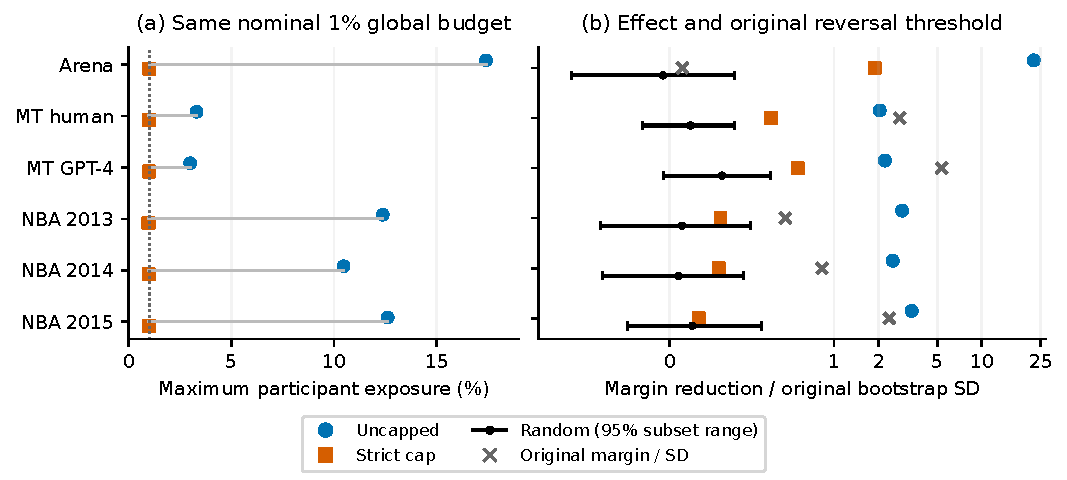
\includegraphics[width=\linewidth]{figures/exposure_response.pdf}
\caption{Primary 1\% audit on six full cohorts. (a) Realized maximum entrant exposure, not the nominal global fraction. (b) Exact margin reductions in original-bootstrap SD units (symlog axis, linear within one unit); crosses mark each original margin/SD, beyond which the fixed pair reverses. Black whiskers are random-subset percentile ranges, not confidence intervals for deterministic attacks. Capped counts can be much smaller (Table~\ref{tab:primary}).}\label{fig:primary}
\end{figure}

\begin{table}[t]
\centering\small
\caption{Nominal 1\% outcome-reversal budget. U: uncapped; C: strict capped greedy. $k$: actual edits; $\rho_U$: maximum entrant exposure; $D$: exact reduction/original bootstrap SD. Last column is reversal frequency over 100 random subsets, not a worst-case rate; Wilson intervals are in Table~\ref{tab:uncertainty}.}\label{tab:primary}
\begin{tabular}{lrrrrrr}
\toprule
Cohort & $k_U$ & $100\rho_U$ & $D_U$ & $k_C$ & $D_C$ & Random flip \\
\midrule
Arena & 574 & 17.4 & 22.49 & 555 & 1.88 & 35\% \\
MT human & 33 & 3.3 & 2.04 & 29 & 0.62 & 0\% \\
MT GPT-4 & 24 & 3.0 & 2.21 & 24 & 0.78 & 0\% \\
NBA 2013 & 13 & 12.4 & 2.89 & 1 & 0.31 & 1\% \\
NBA 2014 & 13 & 10.5 & 2.50 & 2 & 0.30 & 0\% \\
NBA 2015 & 13 & 12.6 & 3.36 & 1 & 0.18 & 0\% \\
\bottomrule
\end{tabular}


\end{table}

The sports contrast has a different mechanism. Thirteen global edits correspond to roughly a tenth or more of one team's observed schedule, whereas strict 1\% incident caps leave most teams with zero capacity. Equation~\eqref{eq:countbound} permits at most one, two, and one edits in the respective seasons; the greedy sets attain these count bounds. Smaller capped effects here do not establish that equally many dispersed edits would be harmless: equally many edits are not feasible under that restriction. The cap-plus-one check admits additional edits by \emph{changing} the restriction, and is labeled accordingly (Appendix~\ref{app:stress}).

The integer-linear check attains solver-reported optimality in all tested conditions and gives closely matching capped refit margins. It rules out a large greedy loss in the \emph{tested first-order surrogate}; it does not establish a global optimum of the nonlinear perturbation problem. Figure~\ref{fig:curves} reports complete budget curves rather than selecting a favorable threshold.

\subsection{Point flips, random noise, and original uncertainty differ}
Arena's original margin is only \R{arenamargin}, with percentile interval $[\R{arenacilow},\R{arenacihigh}]$. The original leader remains first in only 52\% of original-data bootstrap replicates. Uniform 1\% random reversals switch the pair in 35\% of runs, while uncapped targeted reversals produce a much larger score change. A random or capped point flip therefore does not, by itself, destroy a well-established original separation. It can coexist with a valid warning that a sufficiently targeted edit changes scores substantially.

In the other full cohorts, random 1\% reversals occur in zero or one of 100 trials; zero observed trials is not a zero-probability conclusion. Targeted reductions are substantially larger than random mean reductions (Figure~\ref{fig:primary}), including where they fail to reverse the pair. The NBA2015 unperturbed interval excludes zero under the game-bootstrap approximation, yet its uncapped 1\% witness reverses the pair. Conversely, MT's larger margins can survive an adversarial reduction of more than two original SDs. A flip count alone misses both distinctions.

\begin{figure}[t]
\centering
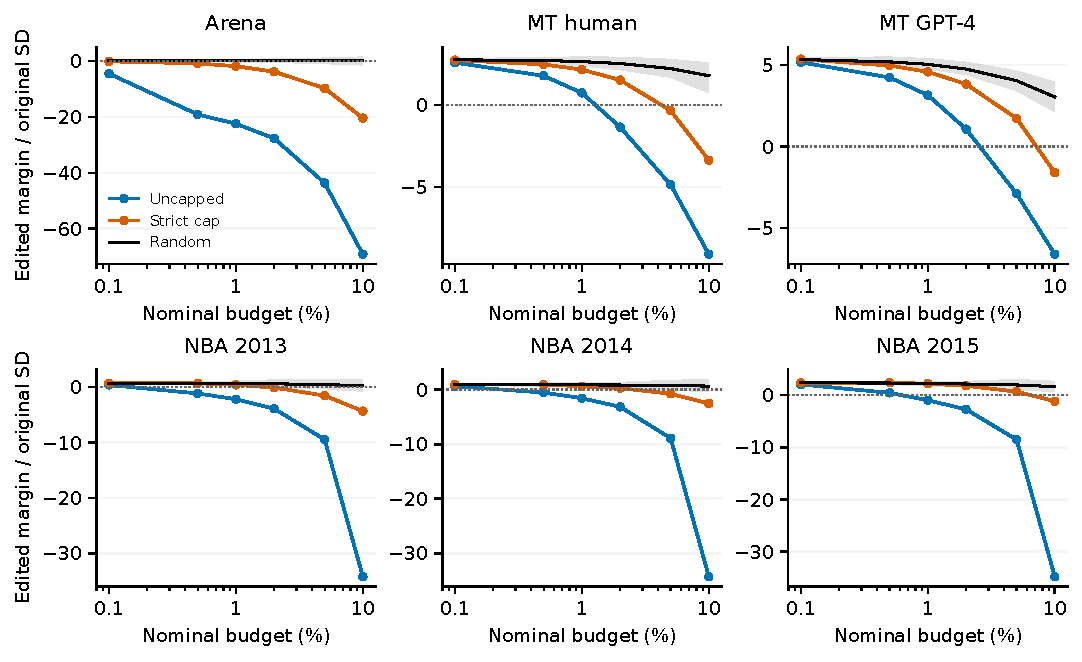
\includegraphics[width=\linewidth]{figures/sensitivity_curves.pdf}
\caption{Budget curves for the fixed original top pair. Vertical scale is margin/original bootstrap SD, with different ranges across panels. Horizontal scale is logarithmic nominal global budget; exact integer counts and strict caps are recomputed at each point. Shading is the empirical 95\% random-subset range. Crossing zero is a point-order reversal, not a significance reversal or a minimum-edit certificate.}\label{fig:curves}
\end{figure}

Exploratory end-to-end resampling retains the large contrast between uncapped and capped reductions but changes the interpretation of individual reversals (Figure~\ref{fig:boot}, Table~\ref{tab:boot}). In particular, Arena's capped edited-margin percentile interval still crosses zero. The selected sets differ across resamples; these distributions are neither repeated attempts at one fixed attack nor guarantees about an unknown population.

\subsection{Matched judges: separation is not the same as response}
The matched panels have exactly the same cells and endpoint degrees. GPT-4's original GPT-4-versus-Claude margin exceeds the human margin by \R{matcheddifference}, with paired question-bootstrap interval $[\R{matchedbootstrapcilow},\R{matchedbootstrapcihigh}]$ (Table~\ref{tab:matched}). Both retain positive margins under the 1\% global edit procedure, although the human panel is much closer to a reversal. Their standardized uncapped reductions, \R{mthumanmatchedinfluencestandardizedreduction} and \R{mtgpt4matchedinfluencestandardizedreduction}, are similar in magnitude. This supports a distinction between initial separation and response to a particular perturbation, not a claim that a model judge is more accurate, less biased, or generally safer.

\begin{table}[t]
\centering\small
\caption{Common MT cells, equal cell weighting, same fixed GPT-4-versus-Claude target. U and C margins follow nominal 1\% \emph{cell} reversals. Cell costs are not interchangeable with full-release judgment costs. Original intervals use synchronized question bootstrap draws.}\label{tab:matched}
\begin{tabular}{lrrrr}
\toprule
Equal-weight panel & $m_0$ & Original interval & $m_U$ & $m_C$ \\
\midrule
MT human (cells) & 0.293 & [0.084, 0.540] & 0.030 & 0.218 \\
MT GPT-4 (cells) & 0.772 & [0.488, 1.099] & 0.428 & 0.670 \\
\bottomrule
\end{tabular}


\end{table}

\subsection{Specification checks expose non-universality}
The main full-cohort reversal pattern persists under the two ridge alternatives, but this is not invariance to the entire modeling pipeline. Dropping exact ties already switches the original Arena top pair \emph{before} editing; attributing that switch to the edit would be incorrect. Excluding inconsistent GPT-4 outcomes and restricting human judge sources change both initial margins and the effective denominators (Tables~\ref{tab:specifications}--\ref{tab:semantics}). Whole-question reversals produce another response curve because a question spans many correlated judgments, rather than being an interchangeable vote (Table~\ref{tab:groups}).

Static and batch-adaptive outcomes, cap rounding, and integer-linear selection are reported together in Table~\ref{tab:stress}. Exact-refit checks are essential: the Arena 1\% deletion control predicts a reduction of about 0.764 but actually reduces the margin by about 2.281. This is finite-perturbation nonlinearity, despite accurate infinitesimal derivatives. Appendix~\ref{app:approx} gives the complete linear-versus-refit diagnostic and grid witnesses without claiming optimal thresholds.

\section{Discussion and limitations}\label{sec:limits}
\paragraph{Scope of the finding.}
The supported claim is not that leaderboards are universally fragile or robust. It is that a global fraction does not specify exposure, and small point-rank changes have different interpretations depending on initial separation and feasible edits. These statements follow from actual counterfactual refits and explicit denominators. The strict-cap comparison is an audit of a different admissible set, not evidence that platforms enforce such caps or that they remove all dangerous perturbations.

\paragraph{Statistical limits.}
The top pair is selected from the same data and held fixed; intervals are descriptive, not winner-selection-adjusted inference. Prompt-string clustering does not recover user dependence, question clustering does not model shared judges across questions, and NBA game resampling does not capture serial, team, home-court, or season dynamics. Static BT may be misspecified, especially for changing sports strengths or nontransitive model preferences. A ridge-finite fit need not be a well-specified generative model. No cross-domain ordering should be interpreted causally, and six full cohorts do not estimate a population prevalence of vulnerable leaderboards.

\paragraph{Perturbation and computational limits.}
We assume offline access to the observed schedule and outcomes. Real manipulation has costs, detection, and access restrictions absent here. Tie reversals, deletions, question edits, and averaged-cell reversals have different semantics. Same-$\lambda$ sum-loss fits have different relative regularization across sample sizes. Static influence and its integer surrogate do not solve the nonlinear minimum-edit problem. Small-budget zeros can be arithmetic restrictions rather than statistical robustness. Optional matched-exposure Arena subsampling was not run; no equal-exposure causal contrast is claimed. The bounded literature protocol prevents an exhaustive claim of originality.

\subsection{Broader impact and research process}\label{sec:impact}
Exposure-aware reporting can help readers avoid unsupported selection and marketing claims. Conversely, edit-selection code could be repurposed to manipulate evaluations or to exaggerate the significance of a harmless near-tie. We release an offline audit with exposure and uncertainty diagnostics, no live-voting integration, no account identification, and no raw conversations in the code archive. These choices reduce operational and privacy risks but are not complete misuse safeguards. No new participants were recruited or identified; all analyses use public licensed historical records. No new institutional review was obtained, and no unverified approval or exemption is asserted. Substantial LLM assistance and the restricted-access protocol are disclosed in the appendix.

\section{Conclusion}
A useful stability report should state \emph{what} is edited, \emph{whose} evidence is affected, \emph{how many} edits are actually feasible, and \emph{which} conclusion changes relative to original uncertainty. On the tested snapshots, global influence-selected reversals, strict exposure caps, and random errors lead to materially different interpretations. Reporting only a small global fraction or a flipped first-place label omits those distinctions. Our evidence is a set of reproducible conditional witnesses and controls, not a universal robustness verdict.

\label{maintextend}
\clearpage
\bibliographystyle{plainnat}
\bibliography{permitted_literature}
\clearpage
\appendix
\section{Objective, derivatives, and counting identities}\label{app:derivation}
Write $L(\theta;y,w)=\sum_r w_r[\log(1+\exp(x_r^\top\theta))-y_rx_r^\top\theta]+\lambda\|\theta\|^2/2$, with all original $w_r=1$ and $\lambda>0$. The gradient and Hessian are
\begin{align}\label{eq:grad}
 g(\theta)&=\sum_r w_rx_r(p_r-y_r)+\lambda\theta,\\
 H(\theta)&=\sum_r w_rp_r(1-p_r)x_rx_r^\top+\lambda I.\label{eq:hessian}
\end{align}
For nonnegative weights, $H$ is positive definite. The loss is smooth and coercive because of the positive quadratic penalty, so a unique finite minimizer exists. Summing the gradient coordinates gives $\lambda\sum_i\widehat\theta_i=0$. This justifies centered coordinates without an arbitrary reference entrant.

For a single record, continuously interpolate its outcome as $y_r(t)=y_r+t(1-2y_r)$, holding weights fixed. Differentiating $g(\widehat\theta(t),t)=0$ at $t=0$ gives
\begin{equation}\label{eq:flipderivative}
 H\frac{d\widehat\theta}{dt}+x_r(2y_r-1)=0,
 \qquad -\frac{dm}{dt}=c^\top H^{-1}x_r(2y_r-1).
\end{equation}
For deletion, use $w_r(t)=1-t$ and fixed response. The corresponding derivative is
\begin{equation}\label{eq:delderivative}
 H\frac{d\widehat\theta}{dt}-x_r(p_r-y_r)=0,
 \qquad -\frac{dm}{dt}=c^\top H^{-1}x_r(y_r-p_r).
\end{equation}
The actual discrete operation uses $t=1$, for which this derivative need not approximate the full refit accurately. Positive-score sorting optimizes only the additive first-order objective. The ridge term remains in the Hessian and is not removed or rescaled after deletion. These standard implicit derivatives are implementation identities, not a novel influence theorem.

For exposure, $\sum_i n_i=2N$ and $\sum_i k_i(S)=2|S|$, because each retained comparison has exactly two distinct endpoints. Substitution proves Eq.~\eqref{eq:exposure}; a weighted average cannot exceed the maximum of its terms. Summing strict capacities and dividing by two proves Eq.~\eqref{eq:countbound}; the integer floor follows because $|S|$ is integral. This count bound does not depend on any fitted score or attack heuristic. It is generally not tight when endpoint pairs, beneficial outcomes, or other constraints limit feasibility.

\paragraph{Numerical implementation.}
We aggregate counts and response sums for each canonical unordered pair; this is exact for Eq.~\eqref{eq:bt}, including fractional responses. Newton steps solve the dense positive-definite system using SciPy, with backtracking and a default maximum gradient target $10^{-8}$. A fit fails if its final gradient exceeds $2\times10^{-6}$ or has a nonfinite state; no such production failure occurred. Canonical orientation is checked at the data boundary because lower-triangle inputs would otherwise be silently omitted by upper-triangle sufficient statistics. Analytical two-player and finite-difference gradient, Hessian, outcome, and deletion tests are supplied, along with integer-surrogate brute force on a toy example. The toy fixture is a unit test, not experimental synthetic evidence.

For the integer-linear control, one bounded integer variable counts selected records in an observed $(a,b,y)$ class; all members have equal influence. Endpoint incidence constraints and a global cardinality constraint are linear. SciPy's mixed-integer solver uses a 60-second limit and relative gap target $10^{-9}$; every recorded condition terminates with status zero and reported gap zero. Refitted margins remain feasible nonlinear witnesses only. Different equal-objective class allocations can produce different discrete sets or counts.

\section{Data snapshots, provenance, and edit semantics}\label{app:data}
The data owners are LMArena/LMSYS for Arena, the MT-Bench authors for the judgment release, and FiveThirtyEight for the NBA archive. We downloaded only the fixed public snapshots specified in the task. Table~\ref{tab:sources} records the commits and terms; the code's \texttt{artifacts/data\_manifest.json} records exact resolve URLs, bytes, and SHA256 values for all four source files. Three supplied hashes are checked before parsing; the fourth (GPT-4 parquet) is computed and recorded. Raw data remain in \texttt{data/} and are excluded from the reproduction archive.

\begin{table}[h]
\centering\small
\caption{Source snapshots. Dataset cards and repository license were fetched directly and retained in the provenance bundle. No third-party rehosting or restricted dataset is needed.}\label{tab:sources}
\begin{tabular}{p{.17\linewidth}p{.57\linewidth}p{.17\linewidth}}
\toprule
Source & Public repository and fixed commit & License\\
\midrule
Arena55k & \url{https://huggingface.co/datasets/lmarena-ai/arena-human-preference-55k}; \texttt{18c298340948c0e7f7727399fd459cca6ce0ca6f} & Apache-2.0\\
MT human / GPT-4 & \url{https://huggingface.co/datasets/lmsys/mt_bench_human_judgments}; \texttt{f7d2896d2cc5d80f8b55c2bbc722613555233c25} & CC-BY-4.0\\
NBA historical & \url{https://github.com/fivethirtyeight/data}; \texttt{4c1ff5e3aef1816ae04af63218015066e186c147}; \texttt{nba-elo/nbaallelo.csv} & CC-BY-4.0\\
\bottomrule
\end{tabular}

\end{table}

Arena uses all eligible rows and all observed models, with no outcome-based top-model trimming. Winner columns are checked to sum to one; self comparisons and invalid winners would be excluded and counted. The retained full snapshot has no such exclusions or duplicate record IDs. Prompt content is used only for exact-string hashing to define resampling clusters; no conversations are quoted or redistributed. The term ``55k'' is the public dataset label rather than the exact retained count in Table~\ref{tab:data}.

MT processing maps observed winner labels to $1,0,0.5$ and canonicalizes model orientation before aggregation. There are 380 GPT-4 records labeled \texttt{tie (inconsistent)}, distinct from 220 explicit ties; the main fit includes both as half outcomes. The human source restrictions select the observed \texttt{expert\_} versus \texttt{author\_} label prefix without inferring identities. \texttt{mt\_human\_cell\_provenance.csv} and its GPT-4 counterpart retain question, turn, unordered pair, multiplicity, number of distinct judges, and source row indices, sufficient to reconstruct each aggregate without redistributing conversations. Each common cell is weighted equally, regardless of its human judgment multiplicity. Matched-cell response reversals invert the entire mean; their nominal cell budgets are not raw-vote budgets.

For NBA, filter league NBA and the three fixed \texttt{year\_id} values, then retain \texttt{\_iscopy==0}. Game IDs are verified unique. A game outcome is one binary comparison; the mirrored opponent row is not a second observation. Historical records are used as a cross-domain test of a static score aggregation, not to infer current team ability, home advantage, or misconduct.

\section{Uncertainty details and additional controls}\label{app:uncertainty}
Each original-data replicate samples the same number of clusters as observed, with replacement, and assigns every row its cluster multiplicity as a likelihood weight. The pair remains fixed to the full-data leader/runner. The base seed is 20261104; original and exploratory bootstraps use seed base $+100000+b$, and random controls use base $+r$ or base $+200000+r$. Random sets at different nominal budgets share a permutation within a seed and are therefore nested, not independent across the budget curve. This coupling is deliberate and is not used for multiplicity-unadjusted significance tests.

\begin{table}[h]
\centering\small
\caption{Uncertainty at nominal 1\% on full cohorts. $s_0$: original margin SD. Win retention: original leader remains first under cluster bootstrap. Flip: random-subset pair-reversal frequency with Wilson 95\% interval (100 draws). Last column: empirical 2.5--97.5\% random edited-margin range, not an interval for an estimated mean.}\label{tab:uncertainty}
\begin{tabular}{lrrrrr}
\toprule
Cohort & $s_0$ & Win retain\% & Flip\% & Wilson interval\% & Random margin range \\
\midrule
Arena & 0.055 & 52.0 & 35 & [26.4, 44.7] & [-0.018, 0.038] \\
MT human & 0.136 & 100.0 & 0 & [0.0, 3.7] & [0.325, 0.401] \\
MT GPT-4 & 0.153 & 100.0 & 0 & [0.0, 3.7] & [0.726, 0.826] \\
NBA 2013 & 0.324 & 64.7 & 1 & [0.2, 5.4] & [0.069, 0.364] \\
NBA 2014 & 0.318 & 78.3 & 0 & [0.0, 3.7] & [0.152, 0.426] \\
NBA 2015 & 0.314 & 96.7 & 0 & [0.0, 3.7] & [0.568, 0.825] \\
\bottomrule
\end{tabular}


\end{table}

The count-matched control samples exactly as many non-tie records as the corresponding capped greedy set, without enforcing its endpoint restriction. Table~\ref{tab:controls} reports both supplementary random controls. The cap-feasible control shuffles priorities and accepts records greedily if both endpoint slots remain. It is a heuristic feasible sampler, not a uniform distribution over feasible sets or an equal-count control. Reporting their actual mean counts and exposure avoids conflating those roles.

\begin{table}[h]
\centering\small
\caption{Supplementary random controls at nominal 1\%. $D$ uses the same original SD as the primary analysis. Cap-feasible draws can underfill; count-matched draws need not satisfy the caps.}\label{tab:controls}
\begin{tabular}{llrrrr}
\toprule
Cohort & Random control & Mean edits & Mean $100\rho$ & Mean $D$ & 95\% subset range \\
\midrule
Arena & Count-matched & 555.0 & 2.07 & -0.014 & [-0.430, 0.413] \\
Arena & Cap-feasible & 557.0 & 1.00 & -0.020 & [-0.464, 0.365] \\
MT human & Count-matched & 29.0 & 1.19 & 0.085 & [-0.145, 0.320] \\
MT human & Cap-feasible & 31.2 & 0.99 & 0.107 & [-0.129, 0.338] \\
MT GPT-4 & Count-matched & 24.0 & 1.41 & 0.276 & [-0.029, 0.594] \\
MT GPT-4 & Cap-feasible & 23.4 & 1.00 & 0.247 & [0.003, 0.417] \\
NBA 2013 & Count-matched & 1.0 & 1.19 & 0.002 & [-0.138, 0.161] \\
NBA 2013 & Cap-feasible & 1.0 & 0.99 & 0.037 & [-0.311, 0.309] \\
NBA 2014 & Count-matched & 2.0 & 1.31 & 0.008 & [-0.140, 0.158] \\
NBA 2014 & Cap-feasible & 2.0 & 0.99 & -0.008 & [-0.300, 0.298] \\
NBA 2015 & Count-matched & 1.0 & 1.19 & 0.007 & [-0.144, 0.188] \\
NBA 2015 & Cap-feasible & 1.0 & 0.98 & 0.072 & [-0.182, 0.175] \\
\bottomrule
\end{tabular}


\end{table}

\paragraph{Matched contrast.}
The common panels contain the same question IDs and cell order; matching is by question, turn, and unordered pair. Synchronized bootstrap question draws therefore support a paired difference of the \emph{same} GPT-4-versus-Claude margin. This difference does not establish evaluator accuracy: there is no external ground truth for which model should have the larger gap. Unmatched full releases are not substituted for this paired target.

\clearpage
\section{Cap feasibility and specification stress tests}\label{app:stress}
Table~\ref{tab:feasibility} separates endpoint-slot arithmetic from the selected procedure's behavior. Table~\ref{tab:stress} compares the tested selection and rounding variants.
\begin{table}[h]
\centering\small
\caption{Primary strict-cap arithmetic. Eligible rows are non-ties whose two endpoints have positive capacities, before considering their influence signs. Count upper bound is Eq.~\eqref{eq:countbound}; edges may reduce feasibility further. In NBA this upper bound already explains the one/two/one selected counts.}\label{tab:feasibility}
\begin{tabular}{lrrrrr}
\toprule
Cohort & Global budget & Zero-cap entrants & Eligible rows & Count upper bound & Greedy edits \\
\midrule
Arena & 574 & 0 & 39716 & 559 & 555 \\
MT human & 33 & 0 & 2575 & 32 & 29 \\
MT GPT-4 & 24 & 0 & 1800 & 24 & 24 \\
NBA 2013 & 13 & 27 & 21 & 1 & 1 \\
NBA 2014 & 13 & 26 & 33 & 2 & 2 \\
NBA 2015 & 13 & 28 & 8 & 1 & 1 \\
\bottomrule
\end{tabular}


\end{table}

\begin{table}[h]
\centering\small
\caption{Exact edited fixed-pair margins at nominal 1\%. Adaptive U uses at most ten batches; Integer C optimizes the additive influence surrogate under strict caps. Cap+1 replaces every endpoint limit by $\lfloor\alpha n_i\rfloor+1$ while keeping the original global budget. Its larger realized $\rho$ demonstrates a changed restriction, not equivalent rounding.}\label{tab:stress}
\begin{tabular}{lrrrrrr}
\toprule
Cohort & Static U & Adaptive U & Greedy C & Integer C & Cap+1 & $100\rho_{{+1}}$ \\
\midrule
Arena & -1.244 & -1.244 & -0.100 & -0.101 & -0.106 & 2.00 \\
MT human & 0.101 & 0.101 & 0.294 & 0.294 & 0.286 & 1.08 \\
MT GPT-4 & 0.482 & 0.482 & 0.700 & 0.700 & 0.686 & 1.12 \\
NBA 2013 & -0.707 & -0.789 & 0.128 & 0.128 & -0.022 & 2.00 \\
NBA 2014 & -0.500 & -0.576 & 0.200 & 0.200 & 0.088 & 1.98 \\
NBA 2015 & -0.309 & -0.342 & 0.689 & 0.689 & 0.560 & 1.96 \\
\bottomrule
\end{tabular}


\end{table}

\begin{table}[h]
\centering\small
\caption{Uncapped 1\% checks retain the original full-cohort pair. Each specification has its own $N$, unedited fit, degrees, and floor budget. A ``Base reversed'' flag means the unedited altered specification already reverses that pair. NBA tie dropping changes no rows; it is intentionally a null ablation.}\label{tab:specifications}
\begin{tabular}{llrrrr}
\toprule
Cohort & Specification & $N$ & Unedited margin & Edited margin & Base reversed \\
\midrule
Arena & Ridge 0.01 & 57477 & 0.004 & -1.245 & 0 \\
Arena & Ridge 1 & 57477 & 0.008 & -1.231 & 0 \\
Arena & Drop exact ties & 39716 & -0.033 & -6.184 & 1 \\
MT human & Ridge 0.01 & 3355 & 0.378 & 0.101 & 0 \\
MT human & Ridge 1 & 3355 & 0.376 & 0.101 & 0 \\
MT human & Drop exact ties & 2575 & 0.532 & 0.208 & 0 \\
MT GPT-4 & Ridge 0.01 & 2400 & 0.821 & 0.482 & 0 \\
MT GPT-4 & Ridge 1 & 2400 & 0.809 & 0.476 & 0 \\
MT GPT-4 & Drop exact ties & 1800 & 1.100 & 0.563 & 0 \\
NBA 2013 & Ridge 0.01 & 1314 & 0.229 & -0.713 & 0 \\
NBA 2013 & Ridge 1 & 1314 & 0.219 & -0.652 & 0 \\
NBA 2013 & Drop exact ties & 1314 & 0.228 & -0.707 & 0 \\
NBA 2014 & Ridge 0.01 & 1319 & 0.297 & -0.504 & 0 \\
NBA 2014 & Ridge 1 & 1319 & 0.279 & -0.467 & 0 \\
NBA 2014 & Drop exact ties & 1319 & 0.295 & -0.500 & 0 \\
NBA 2015 & Ridge 0.01 & 1311 & 0.750 & -0.312 & 0 \\
NBA 2015 & Ridge 1 & 1311 & 0.693 & -0.285 & 0 \\
NBA 2015 & Drop exact ties & 1311 & 0.744 & -0.309 & 0 \\
\bottomrule
\end{tabular}


\end{table}

\begin{table}[t]
\centering\small
\caption{Observed judge-source and inconsistency-label sensitivities. U/C denote uncapped/strict capped outcome reversals. Different restrictions change the target record population, not merely an attack algorithm. They are exploratory descriptive checks.}\label{tab:semantics}
\begin{tabular}{llrrrrrr}
\toprule
Cohort & Restriction & $N$ & $m_0$ & U1\% & C1\% & U5\% & C5\% \\
\midrule
MT human & experts only & 2668 & 0.403 & 0.144 & 0.319 & -0.640 & -0.026 \\
MT human & authors only & 687 & 0.255 & -0.069 & 0.198 & -0.838 & -0.163 \\
MT GPT-4 & exclude inconsistent & 2020 & 0.992 & 0.548 & 0.833 & -0.774 & 0.264 \\
\bottomrule
\end{tabular}


\end{table}

Whole-question edits reverse every non-tie judgment in a selected MT question, across all observed pairs and turns. Question influence is the sum of row scores, and questions with beneficial total influence are selected in descending order. The question budget is separate from the changed-judgment budget; ties are touched but unchanged. These group edits are not constrained by the row-level endpoint caps. All costs and final margins are reported rather than equating a question with one vote.

\begin{table}[h]
\centering\small
\caption{MT whole-question reversals. Fractions use all 80 questions or the original full-release row count, respectively. ``Changed judgments'' excludes exact ties; touched-row counts are also retained in the source CSV.}\label{tab:groups}
\begin{tabular}{lrrrrr}
\toprule
Cohort & Questions & Question\% & Changed judgments & Row\% & Margin \\
\midrule
MT human & 1 & 1.25 & 39 & 1.16 & 0.274 \\
MT human & 2 & 2.50 & 88 & 2.62 & 0.173 \\
MT human & 4 & 5.00 & 173 & 5.16 & 0.036 \\
MT human & 8 & 10.00 & 320 & 9.54 & -0.209 \\
MT GPT-4 & 1 & 1.25 & 12 & 0.50 & 0.714 \\
MT GPT-4 & 2 & 2.50 & 26 & 1.08 & 0.615 \\
MT GPT-4 & 4 & 5.00 & 60 & 2.50 & 0.439 \\
MT GPT-4 & 8 & 10.00 & 120 & 5.00 & 0.147 \\
\bottomrule
\end{tabular}


\end{table}

\clearpage
\section{Approximation accuracy and observed grid witnesses}\label{app:approx}
Figure~\ref{fig:approx} audits finite-budget approximation errors; Table~\ref{tab:grid} lists the first observed grid witnesses without claiming minimum budgets.
\begin{figure}[h]
\centering
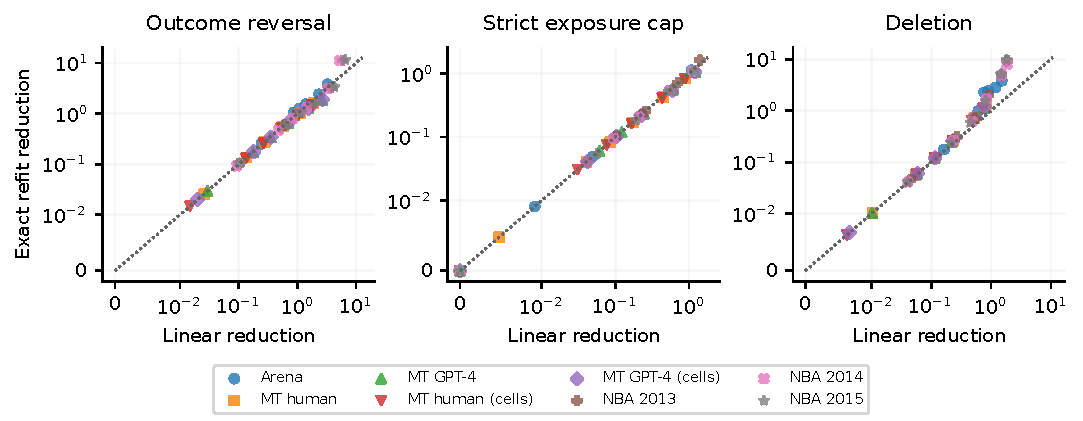
\includegraphics[width=\linewidth]{figures/approximation.pdf}
\caption{Exact-refit versus first-order predicted reductions for every nonzero grid budget and all eight cohorts. Both axes are symlog, linear within 0.01. The dotted line is equality, not a regression. Large finite-budget discrepancies, especially for deletions, preclude using a linearized ranking change as a certificate.}\label{fig:approx}
\end{figure}

\begin{table}[h]
\centering\small
\caption{First \emph{observed} pair reversal on the fixed nominal grid, not the minimum necessary budget. No intermediate budgets or alternative nonlinear edit sets are searched. Matched rows are aggregate-cell units, unlike full-release judgment/game units.}\label{tab:grid}
\begin{tabular}{lrrr}
\toprule
Cohort & Uncapped flip & Capped flip & Deletion \\
\midrule
Arena & 0.1\% & 0.1\% & 0.1\% \\
MT human & 2\% & 5\% & 5\% \\
MT GPT-4 & 5\% & 10\% & 10\% \\
MT human (cells) & 2\% & 5\% & 5\% \\
MT GPT-4 (cells) & 5\% & 10\% & 10\% \\
NBA 2013 & 0.5\% & 2\% & 0.5\% \\
NBA 2014 & 0.5\% & 5\% & 1\% \\
NBA 2015 & 1\% & 10\% & 2\% \\
\bottomrule
\end{tabular}


\end{table}

All deterministic primary and supplementary edit sets have compressed NPZ witnesses containing Unicode row IDs, canonical endpoints, original responses, and selected indices. They are loaded with \texttt{allow\_pickle=False}. The validator reconstructs the appropriate tie/source-restricted data specification and refits from a cold start. It also checks unique indices, exact original responses, nominal global counts, and strict endpoint limits. The current audit replays \R{auditreplayed} deterministic witnesses; the maximum recorded margin discrepancy is below $10^{-7}$. Numerical fit counts and gradients are separately reconciled for the primary, supplemental, and exploratory-bootstrap runs in \texttt{validation.json}. Random sets and bootstrap weights are regenerated from saved seeds and immutable data ordering rather than stored as fabricated witnesses.

\section{Exploratory end-to-end bootstrap}\label{app:boot}
This analysis was added after inspecting the production endpoints, and is explicitly separated from the locked primary plan. For each of 300 cluster draws, expand rows according to cluster multiplicity, refit the unedited data, recompute $N$, entrant degrees, the floor budget, influence ordering, and strict capacities, then select and refit new sets at 1\%. The original full-data contrast is retained, even if already reversed in the unedited resample. All fits use the same ridge as the primary analysis. The intervals describe the entire data-resampling/selection/refitting procedure, not one fixed selected set. No extra replicates were added to shift a percentile endpoint.

\begin{figure}[h]
\centering
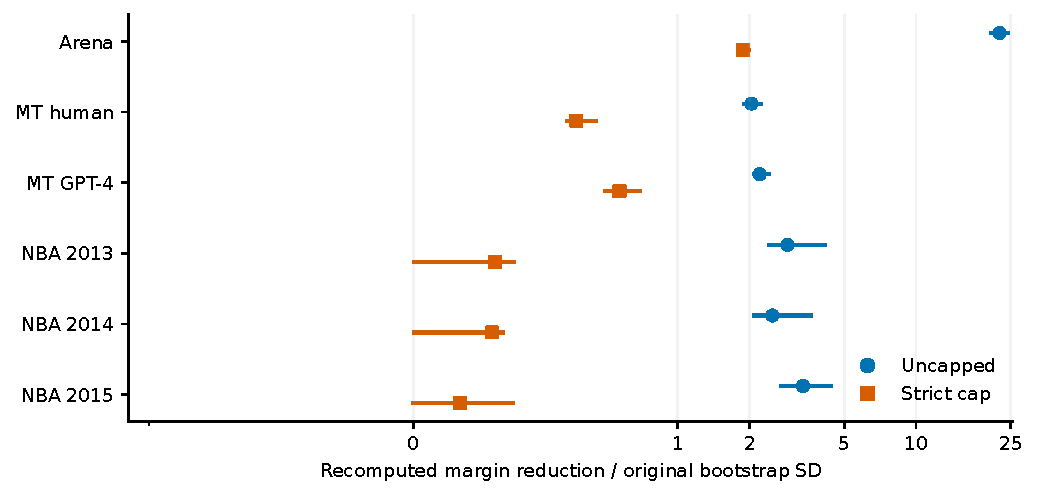
\includegraphics[width=\linewidth]{figures/bootstrap_effects.pdf}
\caption{Exploratory end-to-end effect distributions. Points are original-data reductions; whiskers are percentile reduction ranges from recomputed procedures, divided by the original fixed SD. Symlog horizontal scale is linear within one unit. These are not selection-adjusted intervals or post-edit significance tests.}\label{fig:boot}
\end{figure}

\begin{table}[h]
\centering\small
\caption{Raw-margin percentile intervals for the exploratory recomputed procedure. Reversed\% is the fraction of edited replicate margins below zero, not a frequentist guarantee or a conditional causal effect of editing. It can include resamples with an already reversed original pair.}\label{tab:boot}
\begin{tabular}{llrrr}
\toprule
Cohort & Selector & Reduction interval & Edited-margin interval & Reversed\% \\
\midrule
Arena & U & [1.152, 1.350] & [-1.353, -1.140] & 100.0 \\
Arena & C & [0.101, 0.110] & [-0.209, 0.001] & 97.0 \\
MT human & U & [0.259, 0.305] & [-0.176, 0.382] & 22.7 \\
MT human & C & [0.079, 0.094] & [0.021, 0.574] & 1.0 \\
MT GPT-4 & U & [0.319, 0.370] & [0.215, 0.754] & 0.0 \\
MT GPT-4 & C & [0.111, 0.131] & [0.430, 0.991] & 0.0 \\
NBA 2013 & U & [0.785, 1.339] & [-1.528, -0.190] & 99.3 \\
NBA 2013 & C & [0.001, 0.123] & [-0.486, 0.772] & 33.7 \\
NBA 2014 & U & [0.667, 1.154] & [-1.396, 0.106] & 95.0 \\
NBA 2014 & C & [0.001, 0.108] & [-0.427, 0.853] & 19.3 \\
NBA 2015 & U & [0.855, 1.385] & [-1.070, 0.215] & 87.3 \\
NBA 2015 & C & [0.000, 0.119] & [0.109, 1.326] & 1.0 \\
\bottomrule
\end{tabular}


\end{table}

\clearpage
\section{Reproducibility, compute, and failures}\label{app:reproduce}
The code archive contains \texttt{src/}, \texttt{tests/}, the pinned \texttt{requirements.txt}, \texttt{reproduce.py}, and a README with the data commands and script-to-table/figure map. Run \texttt{python reproduce.py} from the workspace root after installing the requirements; cached original data are checksum-verified. Individual commands are:
\begin{verbatim}
python src/download_data.py
python -m pytest tests -q
python src/run_experiments.py --bootstrap 300 --random 100
python src/run_stress.py --replicates 100
python src/bootstrap_sensitivity.py
python src/validate_results.py
python src/summarize.py
python src/plot_figures.py
python src/complete_checklist.py
latexmk -pdf -cd paper/main.tex
\end{verbatim}
Set \texttt{OPENBLAS\_NUM\_THREADS=1}, \texttt{OMP\_NUM\_THREADS=1}, and \texttt{MKL\_NUM\_THREADS=1} before execution. The numerical environment is Python 3.11.15, NumPy 2.4.6, SciPy 1.17.1, pandas 3.0.6, Matplotlib 3.11.2, PyArrow 26.0.1, pytest 9.2.0, and pypdf 6.21.4. PDF compilation used pdfTeX 1.40.26 (TeX Live 2025/dev/Debian) and the unmodified official NeurIPS 2026 style. The runtime exposes 40 logical CPUs but each numerical process requests one thread; the CPU model and host memory are not exposed through the permitted inspection interface. This does not imply the experiments used 40 cores.

\IfFileExists{resources.tex}{The final replay measured 17.3 seconds for the core experiment process, 17.2 seconds for supplemental controls, and 28.9 seconds for the exploratory bootstrap. The complete download-verification, test, analysis, validation, and rendering sequence took 80.4 seconds before PDF compilation. Peak child resident memory across these stages was 349.5 MiB (Linux cumulative child-process maximum RSS). These are measured times on the provided shared host, not guarantees for another machine. Original pilot and dependency-recovery costs are additional and are logged separately.
}{The machine-readable runtime metadata accompany the code; compilation of this provisional source predates the timed final replay.}

Every scientific CSV can be regenerated without a GPU or paid API. \texttt{summarize.py} produces all numerical tables and the claim ledger; \texttt{plot\_figures.py} reads those CSVs to produce every figure. \texttt{results\_macros.tex} is generated, not a source of invented result numbers. Sufficient-statistic fitting avoids storing a dense $N\times P$ design matrix. Download and TeX/dependency installation time are additional and network-dependent; the budget is comfortably below one CPU week for these snapshots, not a complexity guarantee for larger systems.

\paragraph{Failures and abandoned branches.}
The first NPZ replay failed because object-typed string IDs required unsafe pickle loading; IDs were changed to Unicode and all witnesses regenerated. No unsafe deserialization workaround was used. Initial PDF-extraction dependency recovery and a legacy template URL failure are logged separately; the official 2026 bundle was then obtained from the conference CFP. A blocked system-path CPU-model probe was not bypassed. Optional Arena matched-exposure subsampling was deferred. We did not train manipulation classifiers, call live judges, reproduce a published minimum-edit number, or run a causal evaluator-design experiment. Unsuccessful or unperformed branches are not represented as positive evidence.

\section{LLM assistance, licensing, and access boundaries}\label{app:llm}
An LLM-based research assistant, operating as EvoScientist, autonomously selected the study design, consulted the allowed literature, wrote and tested analysis code, interpreted measured results, and drafted the manuscript. Subagents supplied literature notes, stage critique, and manuscript self-review. The runtime did not expose a verified underlying model identifier; none is invented here. LLM reasoning is not an empirical measurement or mathematical certification: all reported data values, tables, and plotted points are computed by the included CPU programs. No paid inference API, newly generated judge labels, or GPU was used. A human scientific and legal review remains appropriate before actual submission.

New analysis code is supplied under the MIT license; third-party datasets, official style files, and consulted papers retain their original terms. Derived audit summaries and row-ID witnesses do not relicense underlying assets. Raw conversations, all original data files, and third-party paper PDFs are excluded from distribution archives; the source/provenance manifests identify how to obtain them legitimately. The official 2026 checklist is retained with all sixteen answers and justifications.

\subsection{Restricted-access protocol}\label{app:access}
The task specified an unidentified prior paper and prohibited access to it and to pages discussing it, while explicitly permitting a list of starter references. No attempt was made to infer its identity. Literature access was limited to exact permitted arXiv IDs and their own PDFs; no keyword search, citation traversal, related-paper service, review page, or repository search was used. Targeted sections actually read, downloaded versions, hashes, and access failures appear in \texttt{artifacts/literature\_notes.md} and \texttt{access\_and\_failure\_log.md}. This bounded protocol prevents exhaustive novelty clearance. No recognized prohibited source was encountered outside the explicitly permitted set. References printed within permitted PDFs were not followed or used as independently read sources. Later data-card/license, official ethics, and template accesses were exact allowed asset/compliance pages and are logged; no linked further-reading papers were fetched.

\clearpage
\section*{NeurIPS Paper Checklist}




\begin{enumerate}

\item {\bf Claims}
    \item[] Question: Do the main claims made in the abstract and introduction accurately reflect the paper's contributions and scope?
    \item[] Answer: \answerYes{} % Replace by \answerYes{}, \answerNo{}, or \answerNA{}.
    \item[] Justification: Sections~\ref{sec:intro} and~\ref{sec:results} distinguish conditional refit witnesses, exposure restrictions, and uncertainty; no causal design effect or nonlinear optimality is claimed.
    \item[] Guidelines:
    \begin{itemize}
        \item The answer \answerNA{} means that the abstract and introduction do not include the claims made in the paper.
        \item The abstract and/or introduction should clearly state the claims made, including the contributions made in the paper and important assumptions and limitations. A \answerNo{} or \answerNA{} answer to this question will not be perceived well by the reviewers. 
        \item The claims made should match theoretical and experimental results, and reflect how much the results can be expected to generalize to other settings. 
        \item It is fine to include aspirational goals as motivation as long as it is clear that these goals are not attained by the paper. 
    \end{itemize}

\item {\bf Limitations}
    \item[] Question: Does the paper discuss the limitations of the work performed by the authors?
    \item[] Answer: \answerYes{} % Replace by \answerYes{}, \answerNo{}, or \answerNA{}.
    \item[] Justification: Section~\ref{sec:limits} discusses target selection, dependence, model misspecification, edit semantics, integer caps, and restricted novelty clearance.
    \item[] Guidelines:
    \begin{itemize}
        \item The answer \answerNA{} means that the paper has no limitation while the answer \answerNo{} means that the paper has limitations, but those are not discussed in the paper. 
        \item The authors are encouraged to create a separate ``Limitations'' section in their paper.
        \item The paper should point out any strong assumptions and how robust the results are to violations of these assumptions (e.g., independence assumptions, noiseless settings, model well-specification, asymptotic approximations only holding locally). The authors should reflect on how these assumptions might be violated in practice and what the implications would be.
        \item The authors should reflect on the scope of the claims made, e.g., if the approach was only tested on a few datasets or with a few runs. In general, empirical results often depend on implicit assumptions, which should be articulated.
        \item The authors should reflect on the factors that influence the performance of the approach. For example, a facial recognition algorithm may perform poorly when image resolution is low or images are taken in low lighting. Or a speech-to-text system might not be used reliably to provide closed captions for online lectures because it fails to handle technical jargon.
        \item The authors should discuss the computational efficiency of the proposed algorithms and how they scale with dataset size.
        \item If applicable, the authors should discuss possible limitations of their approach to address problems of privacy and fairness.
        \item While the authors might fear that complete honesty about limitations might be used by reviewers as grounds for rejection, a worse outcome might be that reviewers discover limitations that aren't acknowledged in the paper. The authors should use their best judgment and recognize that individual actions in favor of transparency play an important role in developing norms that preserve the integrity of the community. Reviewers will be specifically instructed to not penalize honesty concerning limitations.
    \end{itemize}

\item {\bf Theory assumptions and proofs}
    \item[] Question: For each theoretical result, does the paper provide the full set of assumptions and a complete (and correct) proof?
    \item[] Answer: \answerYes{} % Replace by \answerYes{}, \answerNo{}, or \answerNA{}.
    \item[] Justification: Appendix~\ref{app:derivation} gives the complete objective, positive-ridge assumption, implicit derivative calculation, and elementary exposure-count identities. No novel robustness theorem or certified nonlinear bound is claimed.
    \item[] Guidelines:
    \begin{itemize}
        \item The answer \answerNA{} means that the paper does not include theoretical results. 
        \item All the theorems, formulas, and proofs in the paper should be numbered and cross-referenced.
        \item All assumptions should be clearly stated or referenced in the statement of any theorems.
        \item The proofs can either appear in the main paper or the supplemental material, but if they appear in the supplemental material, the authors are encouraged to provide a short proof sketch to provide intuition. 
        \item Inversely, any informal proof provided in the core of the paper should be complemented by formal proofs provided in appendix or supplemental material.
        \item Theorems and Lemmas that the proof relies upon should be properly referenced. 
    \end{itemize}

    \item {\bf Experimental result reproducibility}
    \item[] Question: Does the paper fully disclose all the information needed to reproduce the main experimental results of the paper to the extent that it affects the main claims and/or conclusions of the paper (regardless of whether the code and data are provided or not)?
    \item[] Answer: \answerYes{} % Replace by \answerYes{}, \answerNo{}, or \answerNA{}.
    \item[] Justification: Section~\ref{sec:setup} and Appendix~\ref{app:reproduce} specify all preprocessing, seeds, optimizers, snapshots, and commands; the accompanying code recreates every figure and table.
    \item[] Guidelines:
    \begin{itemize}
        \item The answer \answerNA{} means that the paper does not include experiments.
        \item If the paper includes experiments, a \answerNo{} answer to this question will not be perceived well by the reviewers: Making the paper reproducible is important, regardless of whether the code and data are provided or not.
        \item If the contribution is a dataset and\slash or model, the authors should describe the steps taken to make their results reproducible or verifiable. 
        \item Depending on the contribution, reproducibility can be accomplished in various ways. For example, if the contribution is a novel architecture, describing the architecture fully might suffice, or if the contribution is a specific model and empirical evaluation, it may be necessary to either make it possible for others to replicate the model with the same dataset, or provide access to the model. In general. releasing code and data is often one good way to accomplish this, but reproducibility can also be provided via detailed instructions for how to replicate the results, access to a hosted model (e.g., in the case of a large language model), releasing of a model checkpoint, or other means that are appropriate to the research performed.
        \item While NeurIPS does not require releasing code, the conference does require all submissions to provide some reasonable avenue for reproducibility, which may depend on the nature of the contribution. For example
        \begin{enumerate}
            \item If the contribution is primarily a new algorithm, the paper should make it clear how to reproduce that algorithm.
            \item If the contribution is primarily a new model architecture, the paper should describe the architecture clearly and fully.
            \item If the contribution is a new model (e.g., a large language model), then there should either be a way to access this model for reproducing the results or a way to reproduce the model (e.g., with an open-source dataset or instructions for how to construct the dataset).
            \item We recognize that reproducibility may be tricky in some cases, in which case authors are welcome to describe the particular way they provide for reproducibility. In the case of closed-source models, it may be that access to the model is limited in some way (e.g., to registered users), but it should be possible for other researchers to have some path to reproducing or verifying the results.
        \end{enumerate}
    \end{itemize}


\item {\bf Open access to data and code}
    \item[] Question: Does the paper provide open access to the data and code, with sufficient instructions to faithfully reproduce the main experimental results, as described in supplemental material?
    \item[] Answer: \answerYes{} % Replace by \answerYes{}, \answerNo{}, or \answerNA{}.
    \item[] Justification: The accompanying reproducibility archive contains all analysis code and exact public-data download commands, with versions and SHA256 hashes (Appendix~\ref{app:reproduce}); raw conversations are not redistributed.
    \item[] Guidelines:
    \begin{itemize}
        \item The answer \answerNA{} means that paper does not include experiments requiring code.
        \item Please see the NeurIPS code and data submission guidelines (\url{https://neurips.cc/public/guides/CodeSubmissionPolicy}) for more details.
        \item While we encourage the release of code and data, we understand that this might not be possible, so \answerNo{} is an acceptable answer. Papers cannot be rejected simply for not including code, unless this is central to the contribution (e.g., for a new open-source benchmark).
        \item The instructions should contain the exact command and environment needed to run to reproduce the results. See the NeurIPS code and data submission guidelines (\url{https://neurips.cc/public/guides/CodeSubmissionPolicy}) for more details.
        \item The authors should provide instructions on data access and preparation, including how to access the raw data, preprocessed data, intermediate data, and generated data, etc.
        \item The authors should provide scripts to reproduce all experimental results for the new proposed method and baselines. If only a subset of experiments are reproducible, they should state which ones are omitted from the script and why.
        \item At submission time, to preserve anonymity, the authors should release anonymized versions (if applicable).
        \item Providing as much information as possible in supplemental material (appended to the paper) is recommended, but including URLs to data and code is permitted.
    \end{itemize}


\item {\bf Experimental setting/details}
    \item[] Question: Does the paper specify all the training and test details (e.g., data splits, hyperparameters, how they were chosen, type of optimizer) necessary to understand the results?
    \item[] Answer: \answerYes{} % Replace by \answerYes{}, \answerNo{}, or \answerNA{}.
    \item[] Justification: Sections~\ref{sec:method}--\ref{sec:setup} specify the fixed-snapshot estimand, ridge, tie policy, budgets, bootstrap clustering, and random controls. There is no predictive train/test split or learned attack classifier.
    \item[] Guidelines:
    \begin{itemize}
        \item The answer \answerNA{} means that the paper does not include experiments.
        \item The experimental setting should be presented in the core of the paper to a level of detail that is necessary to appreciate the results and make sense of them.
        \item The full details can be provided either with the code, in appendix, or as supplemental material.
    \end{itemize}

\item {\bf Experiment statistical significance}
    \item[] Question: Does the paper report error bars suitably and correctly defined or other appropriate information about the statistical significance of the experiments?
    \item[] Answer: \answerYes{} % Replace by \answerYes{}, \answerNo{}, or \answerNA{}.
    \item[] Justification: Tables~\ref{tab:data} and~\ref{tab:uncertainty}, Figures~\ref{fig:curves} and~\ref{fig:boot}, and Section~\ref{sec:uncertainty} separate cluster-bootstrap intervals, random-subset variability, and Wilson Monte Carlo intervals; selection/dependence caveats are explicit.
    \item[] Guidelines:
    \begin{itemize}
        \item The answer \answerNA{} means that the paper does not include experiments.
        \item The authors should answer \answerYes{} if the results are accompanied by error bars, confidence intervals, or statistical significance tests, at least for the experiments that support the main claims of the paper.
        \item The factors of variability that the error bars are capturing should be clearly stated (for example, train/test split, initialization, random drawing of some parameter, or overall run with given experimental conditions).
        \item The method for calculating the error bars should be explained (closed form formula, call to a library function, bootstrap, etc.)
        \item The assumptions made should be given (e.g., Normally distributed errors).
        \item It should be clear whether the error bar is the standard deviation or the standard error of the mean.
        \item It is OK to report 1-sigma error bars, but one should state it. The authors should preferably report a 2-sigma error bar than state that they have a 96\% CI, if the hypothesis of Normality of errors is not verified.
        \item For asymmetric distributions, the authors should be careful not to show in tables or figures symmetric error bars that would yield results that are out of range (e.g., negative error rates).
        \item If error bars are reported in tables or plots, the authors should explain in the text how they were calculated and reference the corresponding figures or tables in the text.
    \end{itemize}

\item {\bf Experiments compute resources}
    \item[] Question: For each experiment, does the paper provide sufficient information on the computer resources (type of compute workers, memory, time of execution) needed to reproduce the experiments?
    \item[] Answer: \answerYes{} % Replace by \answerYes{}, \answerNo{}, or \answerNA{}.
    \item[] Justification: Appendix~\ref{app:reproduce} and the accompanying metadata report CPU-only execution, numerical-library versions, thread settings, measured runtimes, memory, and preliminary/failure logs.
    \item[] Guidelines:
    \begin{itemize}
        \item The answer \answerNA{} means that the paper does not include experiments.
        \item The paper should indicate the type of compute workers CPU or GPU, internal cluster, or cloud provider, including relevant memory and storage.
        \item The paper should provide the amount of compute required for each of the individual experimental runs as well as estimate the total compute. 
        \item The paper should disclose whether the full research project required more compute than the experiments reported in the paper (e.g., preliminary or failed experiments that didn't make it into the paper). 
    \end{itemize}
    
\item {\bf Code of ethics}
    \item[] Question: Does the research conducted in the paper conform, in every respect, with the NeurIPS Code of Ethics \url{https://neurips.cc/public/EthicsGuidelines}?
    \item[] Answer: \answerYes{} % Replace by \answerYes{}, \answerNo{}, or \answerNA{}.
    \item[] Justification: The official Code of Ethics was consulted. Section~\ref{sec:impact} explains public-data secondary analysis, privacy minimization, absence of live manipulation, license compliance, and responsible interpretation.
    \item[] Guidelines:
    \begin{itemize}
        \item The answer \answerNA{} means that the authors have not reviewed the NeurIPS Code of Ethics.
        \item If the authors answer \answerNo, they should explain the special circumstances that require a deviation from the Code of Ethics.
        \item The authors should make sure to preserve anonymity (e.g., if there is a special consideration due to laws or regulations in their jurisdiction).
    \end{itemize}


\item {\bf Broader impacts}
    \item[] Question: Does the paper discuss both potential positive societal impacts and negative societal impacts of the work performed?
    \item[] Answer: \answerYes{} % Replace by \answerYes{}, \answerNo{}, or \answerNA{}.
    \item[] Justification: Section~\ref{sec:impact} discusses improved evaluation transparency, possible misuse for manipulating rankings or misleading publicity, and limits on operational misuse.
    \item[] Guidelines:
    \begin{itemize}
        \item The answer \answerNA{} means that there is no societal impact of the work performed.
        \item If the authors answer \answerNA{} or \answerNo, they should explain why their work has no societal impact or why the paper does not address societal impact.
        \item Examples of negative societal impacts include potential malicious or unintended uses (e.g., disinformation, generating fake profiles, surveillance), fairness considerations (e.g., deployment of technologies that could make decisions that unfairly impact specific groups), privacy considerations, and security considerations.
        \item The conference expects that many papers will be foundational research and not tied to particular applications, let alone deployments. However, if there is a direct path to any negative applications, the authors should point it out. For example, it is legitimate to point out that an improvement in the quality of generative models could be used to generate Deepfakes for disinformation. On the other hand, it is not needed to point out that a generic algorithm for optimizing neural networks could enable people to train models that generate Deepfakes faster.
        \item The authors should consider possible harms that could arise when the technology is being used as intended and functioning correctly, harms that could arise when the technology is being used as intended but gives incorrect results, and harms following from (intentional or unintentional) misuse of the technology.
        \item If there are negative societal impacts, the authors could also discuss possible mitigation strategies (e.g., gated release of models, providing defenses in addition to attacks, mechanisms for monitoring misuse, mechanisms to monitor how a system learns from feedback over time, improving the efficiency and accessibility of ML).
    \end{itemize}
    
\item {\bf Safeguards}
    \item[] Question: Does the paper describe safeguards that have been put in place for responsible release of data or models that have a high risk for misuse (e.g., pre-trained language models, image generators, or scraped datasets)?
    \item[] Answer: \answerYes{} % Replace by \answerYes{}, \answerNo{}, or \answerNA{}.
    \item[] Justification: Section~\ref{sec:impact} describes offline-only edits, no identity inference or live-voting integration, and exclusion of raw conversations from distribution. The code remains dual-use; these measures do not prevent all misuse.
    \item[] Guidelines:
    \begin{itemize}
        \item The answer \answerNA{} means that the paper poses no such risks.
        \item Released models that have a high risk for misuse or dual-use should be released with necessary safeguards to allow for controlled use of the model, for example by requiring that users adhere to usage guidelines or restrictions to access the model or implementing safety filters. 
        \item Datasets that have been scraped from the Internet could pose safety risks. The authors should describe how they avoided releasing unsafe images.
        \item We recognize that providing effective safeguards is challenging, and many papers do not require this, but we encourage authors to take this into account and make a best faith effort.
    \end{itemize}

\item {\bf Licenses for existing assets}
    \item[] Question: Are the creators or original owners of assets (e.g., code, data, models), used in the paper, properly credited and are the license and terms of use explicitly mentioned and properly respected?
    \item[] Answer: \answerYes{} % Replace by \answerYes{}, \answerNo{}, or \answerNA{}.
    \item[] Justification: Appendix~\ref{app:data} credits LMSYS/LMArena and FiveThirtyEight, lists Apache-2.0 and CC-BY-4.0 terms and fixed commits, and preserves official template provenance; third-party assets retain their licenses.
    \item[] Guidelines:
    \begin{itemize}
        \item The answer \answerNA{} means that the paper does not use existing assets.
        \item The authors should cite the original paper that produced the code package or dataset.
        \item The authors should state which version of the asset is used and, if possible, include a URL.
        \item The name of the license (e.g., CC-BY 4.0) should be included for each asset.
        \item For scraped data from a particular source (e.g., website), the copyright and terms of service of that source should be provided.
        \item If assets are released, the license, copyright information, and terms of use in the package should be provided. For popular datasets, \url{paperswithcode.com/datasets} has curated licenses for some datasets. Their licensing guide can help determine the license of a dataset.
        \item For existing datasets that are re-packaged, both the original license and the license of the derived asset (if it has changed) should be provided.
        \item If this information is not available online, the authors are encouraged to reach out to the asset's creators.
    \end{itemize}

\item {\bf New assets}
    \item[] Question: Are new assets introduced in the paper well documented and is the documentation provided alongside the assets?
    \item[] Answer: \answerYes{} % Replace by \answerYes{}, \answerNo{}, or \answerNA{}.
    \item[] Justification: The only new assets are code, derived numerical summaries, and replay witnesses, documented in the accompanying README, artifact map, and code license. No new human data or model weights are released.
    \item[] Guidelines:
    \begin{itemize}
        \item The answer \answerNA{} means that the paper does not release new assets.
        \item Researchers should communicate the details of the dataset\slash code\slash model as part of their submissions via structured templates. This includes details about training, license, limitations, etc. 
        \item The paper should discuss whether and how consent was obtained from people whose asset is used.
        \item At submission time, remember to anonymize your assets (if applicable). You can either create an anonymized URL or include an anonymized zip file.
    \end{itemize}

\item {\bf Crowdsourcing and research with human subjects}
    \item[] Question: For crowdsourcing experiments and research with human subjects, does the paper include the full text of instructions given to participants and screenshots, if applicable, as well as details about compensation (if any)? 
    \item[] Answer: \answerNA{} % Replace by \answerYes{}, \answerNo{}, or \answerNA{}.
    \item[] Justification: No new participants were recruited, paid, or instructed. This study reuses previously released public judgments and games; it makes no claim to re-audit the original collection compensation.
    \item[] Guidelines:
    \begin{itemize}
        \item The answer \answerNA{} means that the paper does not involve crowdsourcing nor research with human subjects.
        \item Including this information in the supplemental material is fine, but if the main contribution of the paper involves human subjects, then as much detail as possible should be included in the main paper. 
        \item According to the NeurIPS Code of Ethics, workers involved in data collection, curation, or other labor should be paid at least the minimum wage in the country of the data collector. 
    \end{itemize}

\item {\bf Institutional review board (IRB) approvals or equivalent for research with human subjects}
    \item[] Question: Does the paper describe potential risks incurred by study participants, whether such risks were disclosed to the subjects, and whether Institutional Review Board (IRB) approvals (or an equivalent approval/review based on the requirements of your country or institution) were obtained?
    \item[] Answer: \answerNA{} % Replace by \answerYes{}, \answerNo{}, or \answerNA{}.
    \item[] Justification: This is secondary analysis of public released records without participant interaction or attempted identification. No new institutional approval was sought, and no claim of exemption or prior approval is fabricated (Section~\ref{sec:impact}).
    \item[] Guidelines:
    \begin{itemize}
        \item The answer \answerNA{} means that the paper does not involve crowdsourcing nor research with human subjects.
        \item Depending on the country in which research is conducted, IRB approval (or equivalent) may be required for any human subjects research. If you obtained IRB approval, you should clearly state this in the paper. 
        \item We recognize that the procedures for this may vary significantly between institutions and locations, and we expect authors to adhere to the NeurIPS Code of Ethics and the guidelines for their institution. 
        \item For initial submissions, do not include any information that would break anonymity (if applicable), such as the institution conducting the review.
    \end{itemize}

\item {\bf Declaration of LLM usage}
    \item[] Question: Does the paper describe the usage of LLMs if it is an important, original, or non-standard component of the core methods in this research? Note that if the LLM is used only for writing, editing, or formatting purposes and does \emph{not} impact the core methodology, scientific rigor, or originality of the research, declaration is not required.
    %this research? 
    \item[] Answer: \answerYes{} % Replace by \answerYes{}, \answerNo{}, or \answerNA{}.
    \item[] Justification: Appendix~\ref{app:llm} discloses substantial LLM assistance in study planning, literature reading, implementation, interpretation, and manuscript preparation; model identity was not exposed by the runtime. All empirical values were computed by the supplied CPU scripts.
    \item[] Guidelines:
    \begin{itemize}
        \item The answer \answerNA{} means that the core method development in this research does not involve LLMs as any important, original, or non-standard components.
        \item Please refer to our LLM policy in the NeurIPS handbook for what should or should not be described.
    \end{itemize}

\end{enumerate}
\end{document}
